\begin{quote}
\textit{The calculus of variations is one of the classical branches of
mathematics. It was Euler who, looking at the work of Lagrange, gave the
present name, not really self explanatory, to this field of mathematics.}\cite[p.~1]{dacorogna}
\end{quote}

In this dissertation, I explore applications of the Direct Method of the Calculus of Variations. Initially, the necessary background and results from functional analysis are introduced in order to establish the mathematical foundation required for the Direct Method. The necessary framework will be developed following Dacorogna’s \textit{Introduction to the Calculus of Variations} \cite{dacorogna}. The Classical Method, based on the Euler–Lagrange equation, is then introduced and applied to simpler variational problems. Building on these results, the Direct Method is explored, forming the principal focus of the dissertation. Finally, the ideas from the Calculus of Variations are applied to a path-planning problem, for which a stochastic numerical solver based on Simulated Annealing is developed to approximate a shortest path between two points. This provides a computational application of the theoretical results developed throughout the dissertation.

{\color{red} Introduction should be longer and more detailed. At its current stage it looks like an abstract of a paper. We should write it at the end, after everything finishes so that we can tell in details what we have done. Don't worry about it now, leave it for the moment.}

\section{Background}

The problems typically associated with the calculus of variations are ancient in comparison with many of the problems considered in modern mathematics, although their formulations can be relatively simple to understand. At its core, the calculus of variations concerns optimisation problems in which one seeks to determine an optimal function with respect to an objective functional. Simple examples include finding the shortest path between two points in a plane or determining the maximum area enclosed by a fixed length of fencing.

Although the formulation of such problems may be relatively straightforward, the methods required to obtain their solutions can be considerably more involved. The development of a systematic framework for the calculus of variations therefore allows more abstract and challenging problems to be considered. One such example is the problem of determining the optimal course of a sailing boat travelling against the wind, as discussed in Rindler’s lecture notes, \textit{Introduction to the Modern Calculus of Variations}.\cite{rindler}

As in many works on the Calculus of Variations, I introduce the subject through Dido’s problem. The semi-historical Phoenician princess, and later and most famously the founder and queen of Carthage, is said to have encountered a variational problem within the founding myth of her city. According to the legend, Dido was offered as much land as could be enclosed by the hide of a bull. She subsequently cut the hide into thin strips and used them to enclose a large area of land, which became the site of Carthage. In doing so, Dido is said to have encountered what is now known as the \textit{isoperimetric problem}: \textit{Find, among all curves of given length, the one which encloses the maximal area} \cite{bandle}.

It was this problem that inspired Euler to seek a general method for solving problems in the Calculus of Variations, laying some of the foundations of the subject. Eleven years after Euler’s work, the nineteen-year-old Lagrange developed a more general method, which impressed Euler \cite{bandle}. The Classical Method of the Calculus of Variations is therefore closely associated with the work of these two mathematical giants. 

Following the development of the Classical Method, what is now known as the Direct Method was conceived through the work of mathematicians including Hilbert, Lebesgue, and Tonelli. Among the problems that motivated this transition was the Dirichlet integral: a problem of multiple integrals \cite{dacorogna}. Hilbert played an important role in the transition of the Calculus of Variations into the modern era, particularly through the 19th, 20th, and 23rd problems that he presented at the International Congress of Mathematicians in Paris in 1900 \cite{rindler}.

This brings us to the present day, where the field of the Calculus of Variations is both broad and active. Mathematicians continue to develop the theory and apply it to an increasingly diverse range of problems, leaving their mark on the subject across areas of both pure and applied mathematics.

{\color{red} This sections looks very good. 

\vspace{2cm}

If I were you I would name the chapters as follows:\\
1. Introduction \\
2. Mathematical modelling\\
3. Numerical methods\\
4. Results\\
5. Conclusion and future work.}

\clearpage

\section{Preliminaries}

In this section, we introduce the foundational mathematics required for the study of the Calculus of Variations. The Classical Method leads to the Euler–Lagrange equation, which transforms a variational problem into an ordinary differential equation. Although the Classical Method is not the primary focus of this dissertation, an understanding of this approach provides useful motivation for the development of the Direct Method.

The Direct Method relies on several results from Functional Analysis, alongside an understanding of $L^p$ and Sobolev spaces. Convexity is also an important tool in analysing variational problems and understanding the properties of their solutions. These concepts provide the mathematical framework required to establish the existence of minimisers using the Direct Method. Establishing existence before applying a numerical method is particularly useful, as it allows us to determine whether a variational problem admits a minimiser before attempting to approximate one computationally.

We now formulate the general form of a Calculus of Variations problem. Throughout this dissertation, we focus primarily on minimisation problems. A general model problem can be written in the form
\begin{equation}
\inf \left\{ I(u) = \int_\Omega f(x,u,\nabla u(x)) \, dx : u \in X \right\} = m,
\tag{P}
\label{eq:General_P}
\end{equation}
where the notation follows the formulation given by Dacorogna \cite[p.~3]{dacorogna}.

Here, the various components of the problem are understood as follows:
\begin{itemize}
    \item $\Omega \subset \mathbb{R}^n$, $n \geq 1$, is a bounded open set, with a point in $\Omega$ denoted by $x = (x_1,\dots,x_n)$;

    \item $u : \Omega \rightarrow \mathbb{R}^N$, $N \geq 1$, is the function being minimised, where
    \[
        u = (u^1,\dots,u^N)
    \]
    and
    \[
        \nabla u =
        \left(
        \frac{\partial u^j}{\partial x_i}
        \right)^{1\leq j\leq N}_{1\leq i\leq n}
        \in \mathbb{R}^{N\times n};
    \]

    \item $f : \overline{\Omega} \times \mathbb{R}^N
    \times \mathbb{R}^{N\times n} \rightarrow \mathbb{R}$ is the integrand, assumed to be continuous;

    \item $X$ denotes the space of admissible functions. For example, one may take
    $X = \{u \in C^1(\overline{\Omega}) : u = u_0 \text{ on } \partial\Omega\}$.
\end{itemize}

We are concerned with finding a \textit{minimiser} $\overline{u} \in X$, 
that is, a function satisfying
\[
    I(\overline{u}) \leq I(u), \qquad \forall u \in X.
\]

All the mathematics we develop will be used with the goal of first proving the existence of minimisers and then searching for potential minimisers for these problems. 

\subsection{The Classical Method}

We begin with a brief overview of the Classical Method, including some examples, in order to establish the ideas that motivate the Direct Method. Following the formulation in Dacorogna \cite[p.~57]{dacorogna}, we consider the one-dimensional variational problem
\begin{equation}
\inf \left\{
I(u): u \in C^1([a,b]),\ u(a)=\alpha,\ u(b)=\beta
\right\},
\tag{P}
\label{eq:Classical_P}
\end{equation}

where $f \in C^2([a,b]\times\mathbb{R}\times\mathbb{R})$ and
\[
    I(u)=\int_a^b f(x,u,u'(x))\,dx.
\]

To motivate the Classical Method, we first recall the analogous minimisation problem in $\mathbb{R}^n$,
\[
\inf\{F(x):x\in X\subset\mathbb{R}^n\}.
\]
For a sufficiently smooth minimiser $\overline{x}$, a necessary condition is
\[
F'(\overline{x})=0.
\]
The second and higher derivatives of $F$ can then be used to investigate the nature of the critical point.

This formulation is a special case of the general variational problem introduced previously. In contrast to the general formulation, the Classical Method considers a one-dimensional domain $[a,b]$ and scalar-valued functions $u:[a,b]\rightarrow\mathbb{R}$. Consequently, the gradient $\nabla u$ is replaced by the ordinary derivative $u'$. The admissible functions are also restricted to $C^1([a,b])$ and are subject to fixed endpoint conditions $u(a)=\alpha$ and $u(b)=\beta$. The endpoint conditions will henceforth be referred to as boundary conditions.

To solve these problems, we can derive the Euler–Lagrange equation that should satisfy any $C^2([a,b])$ minimiser, $\overline{u}$, of $\eqref{eq:Classical_P}$. The Euler–Lagrange equation is analogous to $F'(\overline{x}) = 0$ in $\mathbb{R}^n$. \cite{dacorogna}

The following theorem provides a necessary condition for a sufficiently smooth minimiser of the problem \eqref{eq:Classical_P}. It is stated here in the form used throughout this dissertation; the result corresponds to Theorem 2.1 in Dacorogna \cite[Theorem 2.1, p.~59]{dacorogna}.

\begin{theorem}[Euler--Lagrange equation]
\label{thm:Euler-Lagrange}
    Let $f \in C^2([a,b]\times\mathbb{R}\times\mathbb{R})$, $f = f(x,u,\xi)$, and 
    \begin{equation}
        \inf_{u\in X} \left\{
        I(u) = \int_a^b f(x,u,u'(x))\,dx
        \right\} = m
    \tag{P}
    \label{eq:E-L_P}
    \end{equation}
    where
    \[
    X = \{u \in C^1([a,b]) : u(a)=\alpha,\ u(b)=\beta\}.
    \]
\begin{enumerate}

    \item[(i)] If \eqref{eq:E-L_P} admits a minimiser $\overline{u} \in X \cap C^2[(a,b)]$, then, 
    \begin{equation}
        \frac{d}{dx}[f_\xi(x,\overline{u}(x),\overline{u}'(x))] = f_u(x,\overline{u}(x),\overline{u}'(x))
    \tag{E}
    \label{eq:E-L_E}
    \end{equation}
    
    \item[(ii)] If $\overline{u}$ satisfies \eqref{eq:E-L_E} and if $(u,\xi) \rightarrow f(x,u,\xi)$  is convex for every $x\in[a,b]$, then $\overline{u}$ is a minimiser of \eqref{eq:E-L_P}.

    \item[(iii)] If $(u,\xi) \rightarrow f(x,u,\xi)$  is \textbf{strictly} convex for every $x\in[a,b]$, then the minimiser of \eqref{eq:E-L_P}, if it exists, is unique.
\end{enumerate}

\end{theorem}

\begin{proof}

\begin{enumerate}

    \item[(i)] For every $h \in \mathbb{R}$ and every $v \in C^1[(a,b)]$ with $v(a) = v(b) = 0$ we have
    \[
    I(\overline{u}) \le I(\overline{u} +hv)
    \]
    By setting $\Phi(h) = I(\overline{u} +hv)$, we have that $\Phi \in C^1(\mathbb{R})$ and $\Phi(0) \le \Phi(h)$. We can deduce that $\Phi$ has a relative minimum at $h=0$. So therefore, 
    \[
    \Phi '(0) = \left. \frac{d}{dh}[I(\overline{u} +hv)] \right |_{h=0}=0
    \]
    Noting that
    \[
    \left. \frac{d\Phi}{dh}\right |_{h=0} = \left. \int_a^b \frac{df}{dh}\right |_{h=0} \, dx
    \]
    Differentiating $f(x,u,u')$ with respect to $h$, where $u=\overline{u} + hv$ and $u'=\overline{u}' + hv'$, gives
    \begin{align*}
        \frac{df}{dh} &= \frac{\partial f}{\partial x} \cancel{\frac{dx}{dh}} + \frac{\partial f}{\partial u}\frac{du}{dh} + \frac{\partial f}{\partial \xi}\frac{du'}{dh}\\
        &= \frac{\partial f}{\partial u}v + \frac{\partial f}{\partial \xi}v'
    \end{align*}
    and hence
    \[
       \Phi'(0) = \int_a^b [f_u(x,\overline{u}(x),\overline{u}'(x))v(x) + f_\xi(x,\overline{u}(x),\overline{u}'(x))v'(x)]\, dx = 0
    \]
    Using Integration by Parts on the second term $f_\xi$ we get the following 
    \begin{align*}
        \int_a^b f_\xi(x,\overline{u}(x),\overline{u}'(x))v'(x)\, dx & \\
        = \left[f_\xi(x,\overline{u}(x),\overline{u}'(x))v(x)\right]_a^b &- \int_a^b \left[ \frac{d}{dx}f_\xi(x,\overline{u}(x),\overline{u}'(x)) \right] v(x) \, dx
    \end{align*}
    Since $v(a) = v(b) = 0$ the first term above vanishes. This leaves us with
    \[
    \Phi'(0) = \int_a^b \left[ f_u(x,\overline{u}(x),\overline{u}'(x)) - \frac{d}{dx}f_\xi(x,\overline{u}(x),\overline{u}'(x)) \right] v(x) \, dx = 0
    \]
    Applying the fundamental lemma of the calculus of variations, Theorem~\ref{thm:Fundamental lemma of the calculus of variations}, we have
    \[
        f_u(x,\overline{u}(x),\overline{u}'(x)) - \frac{d}{dx}f_\xi(x,\overline{u}(x),\overline{u}'(x)) = 0
    \]
    which is the Euler-Legrange equation \eqref{eq:E-L_E}.
    \item[(ii)]  to write 
    \item[(iii)] to write 
\end{enumerate}

\end{proof}

We can and will regularly write the Euler--Lagrange equation in its shorter form
\[
f_y - \frac{d}{dx}f_{\xi} = 0
\]

Using Theorem~\ref{thm:Euler-Lagrange}, we can obtain minimisers for one-dimensional variational problems. We now consider several examples, starting with the problem of finding the shortest curve joining two points in the plane. Next, Dido's problem before exploring a counterexample that shows the limitation of the Classical Method to be used as motivation for the development of the Direct Method. 

\begin{example}
\label{ex:straight-line}
Find the shortest curve joining the points$A=(x_a,y_a)$ and $B=(x_b,y_b)$ in the plane, where $x_a<x_b$. We begin with the variational functional for arc length,
\[
J(y)=\int_{x_a}^{x_b}\sqrt{1+(y'(x))^2}\,dx.
\]
The integrand is
\[
f(x,y,\xi)=\sqrt{1+\xi^2},
\]
which is independent of $x$ and $y$. In particular,
$f_y=0$, so the Euler--Lagrange equation \eqref{eq:E-L_E} reduces to
\[
\frac{d}{dx}f_{y'}(x,y(x),y'(x))=0.
\]
Differentiating $f$ with respect to $y'$ gives
\[
f_{y'}(x,y(x),y'(x)) = \frac{y'(x)}{\sqrt{1+(y'(x))^2}}.
\]
Hence, by the reduced Euler--Lagrange equation, $f_{y'}$ is constant on $[x_a,x_b]$. Since
\[
\frac{y'}{\sqrt{1+(y')^2}}
\]
is a strictly increasing function of $y'$, it follows that $y'$ is constant. Therefore,
\[
y(x)=c_1x+c_2,
\]
for constants $c_1,c_2\in\mathbb{R}$. Thus, the extremal is a straight line, as expected.
\end{example}

\begin{example}[Dido's problem]
\label{ex:Dido's problem}
As discussed previously, Dido's problem concerns finding a curve of prescribed length that encloses the maximum possible area. This problem can be formulated variationally as follows.

Among all sufficiently smooth functions $y$ that are positive on $(0,\ell)$ and satisfy $y(0)=y(\ell)=0$, find a function that minimises
\[
J(y) = -\int_0^{\ell}y(x)\sqrt{1-(y'(x))^2} \, dx
\]
The derivation for this formulation can be found at the appendix (yet to write). The Integrand is
\[
f(x,y,\xi) = -y\sqrt{1-\xi^2}
\]
Since $f$ does not explicitly depend on $x$ we can use another reduced form of the Euler--Lagrange equation \eqref{eq:E-L_E}, 
\[
f-\xi f_\xi = \text{constant}
\]
Substituting our integrand into this reduced Euler--Lagrange equation gives the following
\begin{align*}
 f-y' f_{\xi} &\iff -y\sqrt{1-y'^2} -y' \left(\frac{yy'}{\sqrt{1-y'^2}}\right) = c\\
 &\iff y\sqrt{1-y'^2} + y' \left(\frac{yy'}{\sqrt{1-y'^2}}\right) = \overline{c}\\
 &\iff y(1-y'^2) + yy'^2 = \overline{c}\sqrt{1-y'^2}\\
 &\iff y = \overline{c}\sqrt{1-y'^2}\\
 &\iff \overline{c}y' = \pm\sqrt{\overline{c}^2 - y^2} \quad \text{if $\overline{c} \neq 0$, $y = 0$ otherwise.}
\end{align*}
We now have a ODE to solve, by separation of variables we have,
\[
\int \frac{\overline{c}}{\sqrt{\overline{c}^2 - y^2}} \, dy = \pm \int \, dx
\]
Using a substitution of $y(u) = \overline{c}\sin(u) \implies dy = \overline{c}\cos(u) \,du$ on the left hand side,
\[
\int \frac{\overline{c}}{\sqrt{\overline{c}^2 - y^2}} \, dy = \int \frac{\overline{c}^2\cos(u)}{\overline{c}\cos(u)} \, du = \overline{c} u + \tilde{c} 
\]
we therefore obtain 
\[
    x = \overline{c} u + \tilde{c} \implies u = \frac{x}{\overline{c}} + \tilde{c}
\]
for $\overline{c} \neq 0$ we have 
\[
y(x) = \overline{c} \sin (\frac{x}{\overline{c}} + \tilde{c})
\]
as a solution to the variation problem and therefore an extremal. Using our boundary conditions we can find a parametric representation as a solution to the problem.
\[
(x(s),y(s)) = (-\frac{\ell}{\pi}\cos(\frac{\pi}{\ell}s) - \frac{\ell}{\pi}, \frac{\ell}{\pi}\sin(\frac{\pi}{\ell}s))
\]
the derivation of which is beyond the scope of this example.
\begin{figure}[htbp]
    \centering
    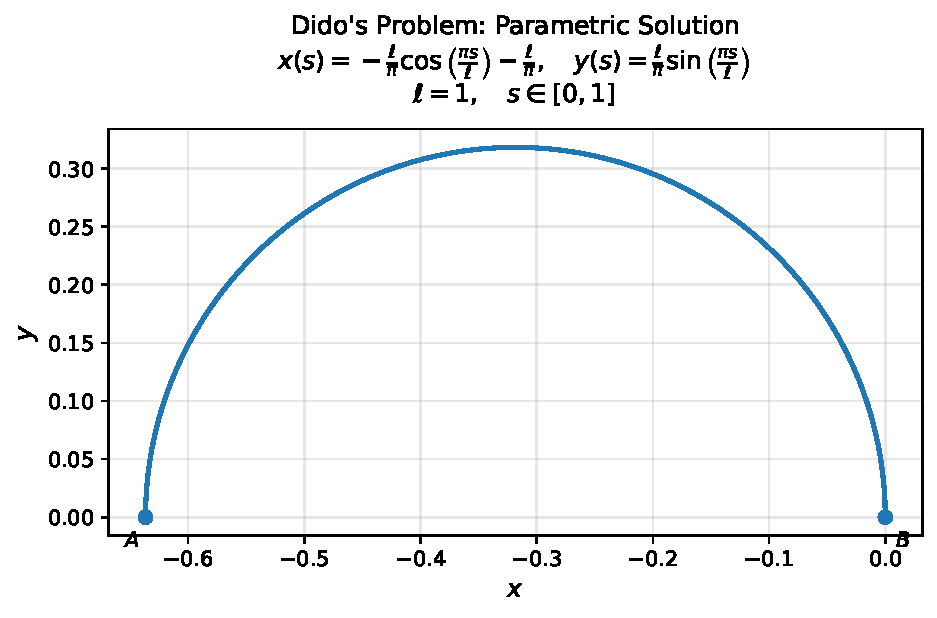
\includegraphics[width=0.7\textwidth]{numerical/outputs/dido.pdf}
    \caption{
        Parametric solution to Dido's problem,
        \[
        x(s)=-\frac{\ell}{\pi}\cos\left(\frac{\pi s}{\ell}\right)
        -\frac{\ell}{\pi},
        \qquad
        y(s)=\frac{\ell}{\pi}\sin\left(\frac{\pi s}{\ell}\right),
        \]
        with $\ell=1$ and $s\in[0,1]$.
    }
    \label{fig:dido-parametric}
\end{figure}
\end{example}

For our counterexample, we consider the Lavrentiev phenomenon and, specifically, the Mani\`a example \cite[p.~70]{dacorogna}. The Euler--Lagrange equation is derived under assumptions on the admissible functions, typically requiring them to be sufficiently smooth ($C^1$ or $C^2$). However, the Mani\`a example demonstrates that a global minimiser of a variational problem need not possess the regularity required by the Classical Method. This motivates the need to consider more general function spaces and provides motivation for the development of the Direct Method.

\begin{example}[Mani\`a Example]
\label{ex:Mania}
Consider the variational problem
\[
J(u)=\int_0^1 (x-u(x)^3)^2(u'(x))^6\,dx.
\]
Subject to the boundary conditions 
\[
u(0) = 0, \qquad u(1) = 1.
\] 
The corresponding integrand is
\[
f(x,u,\xi) = (x-u^3)^2\xi^6
\]
We have the function $\overline{u}(x) = x^{1/3}$ which makes 
\[
J(\overline{u}(x)) = \int_0^1 (x - (x^{1/3})^3)^2\left(\frac{1}{3x^{2/3}}\right)^6 = \int_0^1 0 \, dx = 0  
\]
Since the integrand is non-negative, it follows that
\[
J(u) \geq 0
\]
for every admissible function $u$. Hence $\overline{u}$ is a global minimiser. However the derivative,
\[
\overline{u}'(x)= \frac{1}{3}x^{-2/3}
\]
becomes unbounded as $x \rightarrow 0$. Therefore $\overline{u} \notin C^1([0,1])$. Thus, although $\overline{u}$ is a global minimiser, it does not possess the regularity assumed in the Classical Method. This demonstrates the need to consider broader classes of admissible functions and motivates the development of the Direct Method.
\end{example}


\subsection{Continuous and H\"older Spaces}

We introduce continuous and H\"older spaces following \cite[Section 1.2, p.~14]{dacorogna}, selecting only those results relevant to this dissertation. Additional remarks and explanations are included where useful for developing the ideas required later.

\begin{definition}
    \label{def:Continuous Functions}
    Let $\Omega \subset \mathbb{R}^n$ be an open set.
    \begin{enumerate}
        \item[(ia)] $C^0(\Omega) = C(\Omega)$ is the set of continuous \textbf{functions}, $u : \Omega \rightarrow \mathbb{R}$.
        \item[(ib)] $C^0(\Omega;\mathbb{R}^N) = C(\Omega;\mathbb{R}^N)$ is the set of continuous \textbf{maps}, $u : \Omega \rightarrow \mathbb{R}^N$.
        \item [(ii)] Let $C^0(\overline{\Omega}) = C(\overline{\Omega})$ be the set of continuous functions which can be \textbf{continuously extended} to $\overline{\Omega}$. Similar for maps.
        \item[(iii)] The \textbf{support} of a function $u : \Omega \rightarrow \mathbb{R}$ is defined as 
        \[
            \operatorname{supp} u = \overline{\{x \in \Omega : u(x) \neq 0\}}
        \]
        \item[(iv)] $C_0(\Omega) = \{u \in C(\Omega) : \operatorname{supp} u \subset \Omega \text{ is compact}\}$
        \item[(v)] We define the norm over $C(\overline{\Omega})$ by,
        \[
        \|u\|_{C^0} = \sup_{x \in \overline{\Omega}} |u(x)|
        \]
    \end{enumerate}
\end{definition}

Here are some examples to help build intuition for these definitions.

\begin{example}[Support of a Function]
    \label{ex:Support}

The support of a function is the closure of the region where the function
is \textit{not zero}. Let
\[
u(x) =
\begin{cases}
1-x^2, & \text{if } x\in(-1,1),\\
0, & \text{otherwise}.
\end{cases}
\]

Then:
\begin{itemize}
    \item $u(x)\neq0$ only for $x\in(-1,1)$;

    \item therefore,
    \[
        \{x\in\Omega:u(x)\neq0\}=(-1,1);
    \]

    \item hence, the support is
    \[
        \operatorname{supp}(u)
        =\overline{(-1,1)}
        =[-1,1].
    \]
\end{itemize}

\end{example}

\begin{remark}
    $C(\overline{\Omega})$ equipped with the norm $\|\cdot \|_{C^0}$ is Banach Space
\end{remark}

\begin{theorem}[Ascoli--Arzel\`a theorem]
    \label{thm:Ascoli-Arzela}
    Let $\Omega \subset \mathbb{R}^n$ be a bounded domain. Let $K \subset C(\overline{\Omega})$ be bounded such that the following property of equicontinuity holds: $\forall \varepsilon >0$, there exists $\delta > 0$ 
    \[|x-y| < \delta \implies |u(x) - u(y)| < \varepsilon, \forall x,y \in \overline{\Omega} \text{ and } \forall u\in K \] 
    Then $\overline{K}$ is compact.
\end{theorem}

\begin{example}[Equicontinuity and Ascoli--Arzel\`a]
Consider the sequence of functions on $[0,1]$ given by
\[
    u_n(x)=\frac{x}{n}.
\]
Each $u_n$ is continuous on $[0,1]$, and
\[
    0\leq u_n(x)\leq 1
\]
for all $x\in[0,1]$ and $n\geq1$. Furthermore, for any
$x_1,x_2\in[0,1]$,
\[
    |u_n(x_1)-u_n(x_2)|
    =\frac{1}{n}|x_1-x_2|
    \leq |x_1-x_2|.
\]
Thus, the family $\{u_n\}$ is equicontinuous, since the same bound
controls the change in every function in the family.

The Ascoli--Arzel\`a theorem \ref{thm:Ascoli-Arzela} therefore guarantees that the sequence
contains a uniformly convergent subsequence. In fact, in this example
the whole sequence converges uniformly to the zero function:
\[
    \|u_n\|_{C^0}
    =\sup_{x\in[0,1]}\left|\frac{x}{n}\right|
    =\frac{1}{n}
    \longrightarrow 0.
\]
\end{example}

\begin{remark}
It is important that the hypotheses of the Ascoli--Arzel\`a theorem \ref{thm:Ascoli-Arzela}  are
satisfied. For example, consider
\[
    u_n(x)=x^n,\qquad x\in[0,1].
\]
Although each $u_n$ is continuous and the sequence is uniformly
bounded, the family $\{u_n\}$ is not equicontinuous on $[0,1]$.
Indeed, the functions become increasingly steep near $x=1$.

Pointwise, we have
\[
    u_n(x)\longrightarrow
    \begin{cases}
        0, & 0\leq x<1,\\
        1, & x=1,
    \end{cases}
\]
whose limit is not continuous. Consequently, the sequence cannot have
a uniformly convergent subsequence.
\end{remark}

\begin{remark}
    We introduce the notation for multi-index derivatives, which may not
    be familiar. Let
    \[
        a=(a_1,\dots,a_n)
    \]
    be a multi-index, where each $a_i$ is a non-negative integer. The
    order of $a$ is defined by
    \[
        |a|=a_1+\cdots+a_n.
    \]
    For a sufficiently differentiable function $u:\Omega\to\mathbb{R}$,
    the derivative corresponding to the multi-index $a$ is
    \[
        D^a u
        =
        \frac{\partial^{|a|}u}
        {\partial x_1^{a_1}\cdots\partial x_n^{a_n}}.
    \]
    In other words, $a_i$ tells us how many times to differentiate with
    respect to $x_i$.
\end{remark}

\begin{example}[Multi--Index Derivative]
    \label{ex:multi-index}

    Consider the function
    \[
        u(x,y)=x^2y^3
    \]
    and choose the multi-index
    \[
        a=(1,2).
    \]
    Then
    \[
        D^a u
        =
        \frac{\partial^3 u}{\partial x\,\partial y^2}.
    \]
    Differentiating successively, we obtain
    \[
        u_x=2xy^3,
    \]
    \[
        u_{xy}=6xy^2,
    \]
    and
    \[
        u_{xyy}=12xy.
    \]
    Hence,
    \[
        D^{(1,2)}u=12xy.
    \]
\end{example}

\begin{definition}
    Let $\Omega \subset \mathbb{R}^n$ be an open set and $k\geq0$ be an integer.
    \begin{enumerate}
        \item[(i)] Set of continuous Functions, $u : \Omega \rightarrow \mathbb{R}$, which have all partial derivatives, $D^a u$, $a \in \mathcal{A}_m$, $0 \leq m \leq k$, is $C^k(\Omega)$.
        \item[(ii)] $C^k(\overline{\Omega})$ is the set of functions whose derivatives up to the order $k$ can be extended continuously to $\overline{\Omega}$. It is equipped with the following norm, 
        \[
        \|u\|_{C^k} = \max_{0\leq|a|\leq k} \sup_{x\in\overline{\Omega}}|D^a u(x)|
        \]
        \item[(iii)]  $C^k_0(\Omega) = C^k(\Omega)\cap C_0(\Omega)$

        \item[(iv)]  $C^\infty(\Omega) = \cap_{k=0}^{\infty} C^k(\Omega)$

        \item[(v)]  $C^\infty_0(\Omega) = C^\infty(\Omega) \cap C_0(\Omega)$
    \end{enumerate}
\end{definition}

We now turn to the notion of H\"older continuous functions.

\begin{definition}[H\"older Seminorm]
    \label{def:Holder Semi Norm}
    Let $D \subset \mathbb{R}^n$, $u:D\rightarrow\mathbb{R}$ and
    $0<\alpha\leq1$. The H\"older seminorm of $u$ is defined by
    \[
        [u]_{C^{0,\alpha}(D)}
        =
        \sup_{\substack{x,y\in D\\x\neq y}}
        \frac{|u(x)-u(y)|}{|x-y|^\alpha}.
    \]
\end{definition}

\begin{definition}[H\"older Spaces]
    Let $D\subset\mathbb{R}^n$, $u:D\rightarrow\mathbb{R}$ and
    $0<\alpha\leq1$.
    \begin{enumerate}
        \item[(i)] $C^{0,\alpha}(\Omega)$ is the set of functions
        $u\in C(\Omega)$ such that
        \[
            [u]_{C^{0,\alpha}(K)}<\infty
            \qquad
            \text{for every compact set }K\subset\Omega.
        \]
        \item[(ii)] $C^{0,\alpha}(\overline{\Omega})$ is the set of
        functions $u\in C(\overline{\Omega})$ such that
        \[
            [u]_{C^{0,\alpha}(\overline{\Omega})}<\infty.
        \]
        This space is equipped with the norm
        \[
            \|u\|_{C^{0,\alpha}(\overline{\Omega})}
            =
            \|u\|_{C^0(\overline{\Omega})}
            +
            [u]_{C^{0,\alpha}(\overline{\Omega})}.
        \]
        \item[(iii)] For $k\in\mathbb{N}$, let
        \[
            \mathcal{A}_k
            =
            \{a\in\mathbb{N}_0^n:|a|\leq k\}.
        \]
        Then $C^{k,\alpha}(\Omega)$ is the set of functions
        $u\in C^k(\Omega)$ such that
        \[
            [D^a u]_{C^{0,\alpha}(K)}<\infty
            \qquad
            \text{for every compact set }K\subset\Omega
            \text{ and every }a\in\mathcal{A}_k.
        \]
        \item[(iv)] Similarly,
        $C^{k,\alpha}(\overline{\Omega})$ is the set of functions
        $u\in C^k(\overline{\Omega})$ such that
        \[
            [D^a u]_{C^{0,\alpha}(\overline{\Omega})}<\infty
            \qquad
            \text{for every }a\in\mathcal{A}_k.
        \]
        This space is equipped with the norm
        \[
            \|u\|_{C^{k,\alpha}(\overline{\Omega})}
            =
            \|u\|_{C^k(\overline{\Omega})}
            +
            \max_{a\in\mathcal{A}_k}
            [D^a u]_{C^{0,\alpha}(\overline{\Omega})}.
        \]
    \end{enumerate}
\end{definition}

\begin{remark}[Lipschitz Continuity]
    \label{rem:Lipschitz}
    When $\alpha=1$, the space $C^{0,1}(\overline{\Omega})$ is the space
    of \textit{Lipschitz continuous functions}. In particular, a function
    $u\in C(\overline{\Omega})$ is Lipschitz continuous if there exists a
    constant $\gamma>0$ such that
    \[
        |u(x)-u(y)|
        \leq \gamma |x-y|,
        \qquad
        \forall x,y\in\overline{\Omega}.
    \]
    The smallest possible value of $\gamma$ is given by the H\"older
    seminorm
    \[
        \gamma=[u]_{C^{0,1}(\overline{\Omega})}.
    \]
\end{remark}

\begin{example}[H\"older Continuous Function and Computation of the Norm]
    \label{ex:Holder-norm}

    Let $D=[0,1]$ and define
    \[
        u(x)=\sqrt{x}.
    \]
    We compute the H\"older norm of $u$ in
    $C^{0,\frac{1}{2}}([0,1])$.

    First, the $C^0$ norm is
    \[
        \|u\|_{C^0}
        =
        \sup_{x\in[0,1]}|\sqrt{x}|
        =
        1.
    \]

    Next, taking $\alpha=\frac{1}{2}$, the H\"older seminorm is
    \[
        [u]_{C^{0,\frac{1}{2}}}
        =
        \sup_{\substack{x,y\in[0,1]\\x\neq y}}
        \frac{|\sqrt{x}-\sqrt{y}|}{|x-y|^{1/2}}.
    \]
    Using the identity
    \[
        |\sqrt{x}-\sqrt{y}|
        =
        \frac{|x-y|}{\sqrt{x}+\sqrt{y}},
    \]
    we obtain
    \[
        \frac{|\sqrt{x}-\sqrt{y}|}{|x-y|^{1/2}}
        =
        \frac{|x-y|^{1/2}}{\sqrt{x}+\sqrt{y}}.
    \]
    Without loss of generality, suppose that $x>y$. Then
    \[
        \frac{|x-y|^{1/2}}{\sqrt{x}+\sqrt{y}}
        =
        \frac{\sqrt{x-y}}{\sqrt{x}+\sqrt{y}}
        \leq 1.
    \]
    Equality is attained when $y=0$, giving
    \[
        [u]_{C^{0,\frac{1}{2}}}=1.
    \]

    Therefore, the full H\"older norm is
    \[
        \|u\|_{C^{0,\frac{1}{2}}}
        =
        \|u\|_{C^0}
        +
        [u]_{C^{0,\frac{1}{2}}}
        =
        1+1
        =
        2.
    \]

    This example illustrates that $u(x)=\sqrt{x}$ is continuous but not Lipschitz continuous. 
\end{example}

\begin{example}[$C^{1,\alpha}$ Norm in $\mathbb{R}^2$]
    \label{ex:C1alpha-norm}

    Let $\Omega=[0,1]^2$ and define
    \[
        u(x,y)=x^2+y^2.
    \]
    We illustrate the components of the $C^{1,\alpha}(\Omega)$ norm.

    First, we compute the first partial derivatives:
    \[
        u_x=2x,
        \qquad
        u_y=2y.
    \]

    The $C^1$ norm consists of the supremum norms of the function and
    its first derivatives. We have
    \[
        \sup_{\Omega}|u|=2,
        \qquad
        \sup_{\Omega}|u_x|=2,
        \qquad
        \sup_{\Omega}|u_y|=2.
    \]
    Therefore,
    \[
        \|u\|_{C^1}
        =
        \sup_{\Omega}|u|
        +
        \sup_{\Omega}|u_x|
        +
        \sup_{\Omega}|u_y|
        =
        2+2+2=6.
    \]

    Now consider the H\"older seminorms of the first derivatives. For
    $(x,y),(x',y')\in\Omega$,
    \[
        |u_x(x,y)-u_x(x',y')|
        =
        2|x-x'|
        \leq
        2\|(x,y)-(x',y')\|,
    \]
    and similarly,
    \[
        |u_y(x,y)-u_y(x',y')|
        =
        2|y-y'|
        \leq
        2\|(x,y)-(x',y')\|.
    \]

    In particular, when $\alpha=1$, we have
    \[
        [u_x]_{C^{0,1}(\Omega)}
        =
        [u_y]_{C^{0,1}(\Omega)}
        =2.
    \]
    Hence,
    \[
        \max_{|a|=1}[D^a u]_{C^{0,1}(\Omega)}
        =2.
    \]

    Therefore, using the definition of the $C^{1,1}$ norm,
    \[
        \|u\|_{C^{1,1}(\Omega)}
        =
        \|u\|_{C^1(\Omega)}
        +
        \max_{|a|\leq1}[D^a u]_{C^{0,1}(\Omega)}
    \]
    and, with the convention used here,
    \[
        \|u\|_{C^{1,1}(\Omega)}
        =
        6+2=8.
    \]
\end{example}

\subsection{Lebesgue Spaces}

In this section, we introduce Lebesgue spaces, commonly denoted by $L^p$ spaces. These spaces allow us to work with weaker notions of regularity than those required by the Classical Method, by focusing on the integrability of functions rather than their pointwise smoothness. They are also essential for the definition of Sobolev spaces, which will be introduced in the following section. This provides the language and tools needed to consider whether a function, or its derivatives, are integrable, rather than requiring the stronger pointwise regularity imposed by the Classical Method.

\begin{definition}
    \label{def:L^P Space}
    let $\Omega \subset \mathbb{R}^n$ be an open set and $1 \le p \le \infty$.  We say that a measurable function $u : \Omega \rightarrow \mathbb{R}$ belongs to $L^p(\Omega)$ if $\|u\|_{L^p}$ is finite. For $p$ finite
    \[
    \|u\|_{L^p} = \left(\int_\Omega |u(x)|^p \, dx\right)^{\frac{1}{p}}
    \]   
    And for $p = \infty$
    \[
    \|u\|_{L^p} = \inf\{\alpha : |u(x)<\alpha \text{ a.e. in } \Omega|\}
    \]
\end{definition}

\begin{example}[Example of $L^p$ Norms]
    \label{ex:Lp-norm}

    Let $\Omega=(0,1)$ and define
    \[
        u(x)=x.
    \]

    \begin{enumerate}
        \item[(i)] \textbf{Case $p<\infty$.}

        Consider $p=2$. Then
        \[
            \|u\|_{L^2(0,1)}
            =
            \left(\int_0^1 |x|^2\,dx\right)^{1/2}
            =
            \left(\frac{1}{3}\right)^{1/2}
            =
            \frac{1}{\sqrt{3}}.
        \]
        Since the norm is finite, it follows that
        \[
            u\in L^2(0,1).
        \]

        \item[(ii)] \textbf{Case $p=\infty$.}

        The function $u(x)=x$ takes values arbitrarily close to $1$ on
        $(0,1)$, but does not attain the value $1$. Its essential
        supremum is therefore
        \[
            \|u\|_{L^\infty(0,1)}
            =
            \operatorname*{ess\,sup}_{x\in(0,1)}|u(x)|
            =
            1.
        \]
        Since the essential supremum is finite, it follows that
        \[
            u\in L^\infty(0,1).
        \]
    \end{enumerate}
\end{example}

\begin{example}[A Function in $L^1$ but not in $L^2$]
    \label{ex:L1-not-L2}
    Let
    \[
        u(x)=\frac{1}{\sqrt{x}},
    \]
    defined on $\Omega=(0,1)$. First, consider the $L^1$ norm. We have
    \[
        \|u\|_{L^1(0,1)}
        =
        \int_0^1 |u(x)|\,dx
        =
        \int_0^1 x^{-1/2}\,dx
        =
        2.
    \]
    Hence,
    \[
        u\in L^1(0,1).
    \]
    However, for the $L^2$ norm,
    \[
        \|u\|_{L^2(0,1)}^2
        =
        \left(\int_0^1 |u(x)|^2\,dx\right)^\frac{1}2
        =
        \left(\int_0^1 x^{-1}\,dx\right)^\frac{1}2
        =
        \infty.
    \]
    Therefore,
    \[
        u\notin L^2(0,1).
    \]
    This example illustrates that a function may be integrable in the
    $L^1$ sense without being square-integrable. In particular, membership
    of a function in one $L^p$ space does not automatically imply membership
    in another.
\end{example}

\begin{remark}
    \label{rem:conjugate-exponent}

    In the following theorems, we will make use of the \textit{conjugate
    exponent} of $p$, denoted by $p'$. For $1<p<\infty$, it is defined by
    \[
        \frac{1}{p}+\frac{1}{p'}=1,
        \qquad\text{equivalently}\qquad
        p'=\frac{p}{p-1}.
    \]
    For the endpoint cases, if $p=1$, we define $p'=\infty$, while if $p=\infty$, we define $p'=1$.
\end{remark}

\begin{theorem}[Basic properties of $L^p$ spaces]
    \label{thm:Lebesgue-results}

    Let $\Omega\subset\mathbb{R}^n$ be an open set and let
    $1\leq p\leq\infty$. Then the following hold.

    \begin{enumerate}
        \item[(i)] The space $L^p(\Omega)$ is a Banach space. Moreover,
        $L^2(\Omega)$ is a \textbf{Hilbert space} with inner product
        \[
            \langle u,v\rangle
            =
            \int_{\Omega}u(x)v(x)\,dx.
        \]

        \item[(ii)] \textbf{Hölder's inequality.}
        If $u\in L^p(\Omega)$ and $v\in L^{p'}(\Omega)$, where $p'$ is
        the conjugate exponent of $p$, then $uv\in L^1(\Omega)$ and
        \[
            \|uv\|_{L^1(\Omega)}
            \leq
            \|u\|_{L^p(\Omega)}
            \|v\|_{L^{p'}(\Omega)}.
        \]
        In particular, when $p=p'=2$, this gives the
        \textbf{Cauchy--Schwarz inequality}
        \[
            \|uv\|_{L^1(\Omega)}
            \leq
            \|u\|_{L^2(\Omega)}
            \|v\|_{L^2(\Omega)}.
        \]

        \item[(iii)] \textbf{Minkowski's inequality.}
        If $u,v\in L^p(\Omega)$, then
        \[
            \|u+v\|_{L^p(\Omega)}
            \leq
            \|u\|_{L^p(\Omega)}
            +
            \|v\|_{L^p(\Omega)}.
        \]

        \item[(iv)] \textbf{Duality.}
        If $1\leq p<\infty$ and $\varphi\in(L^p(\Omega))'$, then,
        under the appropriate assumptions, there exists
        $u\in L^{p'}(\Omega)$ such that
        \[
            \langle\varphi,f\rangle
            =
            \varphi(f)
            =
            \int_{\Omega}u(x)f(x)\,dx,
            \qquad
            \forall f\in L^p(\Omega).
        \]

        \item[(v)] The space $L^p(\Omega)$ is separable for
        $1\leq p<\infty$ and reflexive for $1<p<\infty$.

        \item[(vi)] If $1\leq p<\infty$ and $u\in L^p(\Omega)$, then there
        exists a sequence $(u_\nu)\subset C^\infty_0(\Omega)$ such that
        \[
            \lim_{\nu\rightarrow\infty}
            \|u_\nu-u\|_{L^p(\Omega)}
            =
            0.
        \]
        This result is false in general for $p=\infty$.
    \end{enumerate}
\end{theorem}

\begin{remark}[Duality of $L^p$ Spaces]
    \label{rem:Lp-duality}

    To summarise the duality results, we have
    \[
        (L^p(\Omega))' \cong L^{p'}(\Omega),
        \qquad 1<p<\infty,
    \]
    where $p'$ is the conjugate exponent of $p$. In particular,
    \[
        (L^2(\Omega))' \cong L^2(\Omega),
    \]
    since $2'=2$. At the endpoint $p=1$, we have
    \[
        (L^1(\Omega))' \cong L^\infty(\Omega).
    \]
    However, the corresponding result does not hold for $p=\infty$.
    In general,
    \[
        L^1(\Omega)\subsetneq (L^\infty(\Omega))'.
    \]
\end{remark}

We will now consider convergence in $L^p$ spaces. The natural notion of \textit{strong convergence} is induced by the $L^p$ norm. We will also introduce the notion of \textit{weak convergence}, which will be important when considering the Direct Method.

\begin{definition}[Convergence in $L^p$ spaces]
    \label{def:Lp-convergence}

    Let $\Omega\subset\mathbb{R}^n$ be an open set and let
    $1\leq p\leq\infty$.

    \begin{enumerate}
        \item[(i)] A sequence $(u_\nu)$ is said to \textbf{strongly converge}
        to $u$ in $L^p(\Omega)$ if $u_\nu,u\in L^p(\Omega)$ and
        \[
            \lim_{\nu\rightarrow\infty}
            \|u_\nu-u\|_{L^p(\Omega)}
            =0.
        \]
        We denote this by
        \[
            u_\nu\rightarrow u
            \qquad\text{in }L^p(\Omega).
        \]

        \item[(ii)] If $1\leq p<\infty$, a sequence $(u_\nu)$ is said to
        \textbf{weakly converge} to $u$ in $L^p(\Omega)$ if
        $u_\nu,u\in L^p(\Omega)$ and
        \[
            \lim_{\nu\rightarrow\infty}
            \int_\Omega
            [u_\nu(x)-u(x)]\varphi(x)\,\mathrm{d}x
            =0,
            \qquad
            \forall\varphi\in L^{p'}(\Omega).
        \]
        We denote this by
        \[
            u_\nu\rightharpoonup u
            \qquad\text{in }L^p(\Omega).
        \]

        \item[(iii)] If $p=\infty$, a sequence $(u_\nu)$ is said to
        \textbf{weak-$*$ converge} to $u$ in $L^\infty(\Omega)$ if
        $u_\nu,u\in L^\infty(\Omega)$ and
        \[
            \lim_{\nu\rightarrow\infty}
            \int_\Omega
            [u_\nu(x)-u(x)]\varphi(x)\,\mathrm{d}x
            =0,
            \qquad
            \forall\varphi\in L^1(\Omega).
        \]
        We denote this by
        \[
            u_\nu\rightharpoonup^* u
            \qquad\text{in }L^\infty(\Omega).
        \]
    \end{enumerate}
\end{definition}


\begin{example}[Weak Convergence in $L^p$]
    \label{ex:weak-convergence}

    Let $\Omega=(0,1)$ and define
    \[
        u_\nu(x)=\sin(2\pi \nu x).
    \]
    We claim that
    \[
        u_\nu\rightharpoonup 0
        \qquad\text{in }L^p(0,1),
        \qquad 1<p<\infty.
    \]

    Indeed, let $\varphi\in L^{p'}(0,1)$. Then
    \[
        \int_0^1
        u_\nu(x)\varphi(x)\,\mathrm{d}x
        =
        \int_0^1
        \sin(2\pi \nu x)\varphi(x)\,\mathrm{d}x
        \longrightarrow 0
        \qquad\text{as }\nu\rightarrow\infty.
    \]
    This follows from the oscillatory nature of $\sin(2\pi\nu x)$
    and the Riemann--Lebesgue lemma.

    Therefore,
    \[
        u_\nu\rightharpoonup0
        \qquad\text{in }L^p(0,1).
    \]

    However, the convergence is not strong. For example, when $p=2$,
    \[
        \|u_\nu\|_{L^2(0,1)}^2
        =
        \int_0^1\sin^2(2\pi\nu x)\,\mathrm{d}x
        =
        \frac12,
    \]
    and hence
    \[
        \|u_\nu\|_{L^2(0,1)}
        =
        \frac{1}{\sqrt{2}}
        \not\longrightarrow0.
    \]
    Thus, weak convergence does not in general imply strong convergence.
\end{example}

\begin{example}[Weak-$*$ Convergence in $L^\infty$]
    \label{ex:weak-star-convergence}

    Let $\Omega=(0,1)$ and define the sequence $(u_\nu)$ by
    \[
        u_\nu(x)
        =
        (-1)^k,
        \qquad
        x\in
        \left[\frac{k}{\nu},\frac{k+1}{\nu}\right),
        \quad
        k=0,\ldots,\nu-1.
    \]
    Thus, $u_\nu$ alternates between $1$ and $-1$ on increasingly
    fine subintervals of $(0,1)$. In particular,
    \[
        \|u_\nu\|_{L^\infty(0,1)}=1,
    \]
    so the sequence is bounded in $L^\infty(0,1)$.

    For every $\varphi\in L^1(0,1)$, the increasingly rapid oscillations
    of $u_\nu$ imply
    \[
        \int_0^1 u_\nu(x)\varphi(x)\,\mathrm{d}x
        \longrightarrow 0
        \qquad\text{as }\nu\rightarrow\infty.
    \]
    Hence,
    \[
        u_\nu\rightharpoonup^*0
        \qquad\text{in }L^\infty(0,1).
    \]

    However,
    \[
        \|u_\nu-0\|_{L^\infty(0,1)}
        =
        1
    \]
    for every $\nu$. Therefore, $u_\nu$ does not converge strongly to
    zero in $L^\infty(0,1)$.

    This example illustrates that weak-$*$ convergence does not in
    general imply strong convergence in $L^\infty$.
\end{example}

\begin{definition}
    $u \in L^p_{loc}(\Omega)$ if $u \in L^p(\Omega')$ for every open set $\Omega'$ compactly contained in $\Omega$
\end{definition}
\begin{theorem}[Fundamental lemma of the calculus of variations]
\label{thm:Fundamental lemma of the calculus of variations}
Let $\Omega$ be an open set of $\mathbb{R}^n$ and $u \in L^1_{loc}(\Omega)$ be such that 
$$
\int_\Omega u(x)\, \varphi(x) \, \mathrm{d}x = 0, \qquad \forall \varphi \in C^{\infty}_0(\Omega)
$$
then $u = 0$, a.e. in $\Omega$.
\end{theorem}
\begin{proof}
    to write 
\end{proof}

\subsection{Sobolev Spaces}

\subsection{Convex Analysis}
